Static analysis is the process of soundly predicting properties of
programs.
%
It necessarily involves a tradeoff between the precision of those
predictions and the computational complexity of producing them.
%
At one end of the spectrum, an analysis may predict nothing, using no
resources.  At the other end, an analysis may predict everything, at
the cost of computability.

Abstract interpretation~\cite{dvanhorn:Cousot:1977:AI} is a form of
static analysis that involves the \emph{approximate} running of a
program by interpreting a program over an abstraction of the program's
values, e.g. by using intervals in place of
integers~\cite{Cousot-TASE07tutorial}, or types instead of
values~\cite{dvanhorn:esop:kmf07}.
%
By considering the sound abstract interpretation of a program, it is
possible to predict the behavior of concretely running the program. 
%
For example, if abstract running a program never causes a
buffer-overflow, run-time type error, or null-pointer dereference, we
can conclude actually running the program can never cause any of these
errors either.  If a fragment of code is not executed during the
abstract running, it can safely be deemed dead-code and removed.  More
fine-grained properties can be predicted too; to enable inlining, the
abstract running of a program can identify all of the functions that
are called exactly once and the corresponding call-site.  Temporal
properties can be discovered as well: perhaps we want to determine if
one function is always called before another, or if reads from a file
occur within the opening and closing of it.







%% Most static analyses can help find \emph{bugs} but cannot prove their absence (Astr\'ee is perhaps the outlier here).
%% %
%% These analyses can certainly be useful, but they do not cover a topic of ever-increasing importance: security.
%% %
%% Run-time monitors exist for enforcing security policies~\citep{ianjohnson:Erlingsson:2004:IRM:997617}, but fail late and impose significant overhead.
%% %
%% A \emph{sound} analysis that predicts that such run-time monitors never lead to an error state has given us two things:
%% \begin{itemize}
%% \item{\emph{proof} that our program is secure with respect to the monitored properties, and}
%% \item{a guarantee that we can safely remove the run-time monitor to improve performance.}
%% \end{itemize}
%% A \emph{precise} analysis is able to rule out enough spurious behavior that such predictions are actually possible in practice.
%% %
%% An analysis that says,
%% \begin{center}
%%   \textit{Nothing is true, everything is permitted}
%% \end{center}
%% is sound, but is so imprecise that we have learned nothing about the program's behavior. 
%% %
%% If security is not your goal, we still advocate a best-effort-soundness design strategy\footnote{So-called ``soundiness'' (\url{http://soundiness.org})}.

%% The question of sound versus unsound is a question of predicted behavior: are all states a program might find itself in considered?
%% %
%% A programming language semantics is the set of rules that determine how a program state evolves.
%% %
%% If we represent each program state as a node in a graph, and track evolution steps as edges, we get closer to the age-old \emph{control-flow graph} (AKA \emph{flow-chart}), but these concepts are shadows, projections, \emph{approximations} of concrete program behavior.
%% %
%% The art and science of static analysis design is the way we represent this graph of states; how little or how much detail we choose to represent in each state determines the precision and, often, the \emph{cost} of such an analysis.
%% %
%% The AAM methodology for static analysis design is a systematic augmentation of a given programming language semantics; this makes much of static analysis construction mindless boilerplate so that you can focus on your art -- hone in on the novelty of your abstraction.
%% %
%% First-order data-structures, numbers, arrays all have an abundance of literature for precise and effective approximations, so this paper focuses on higher-order data: closures and continuations.
%% %

In general, we can model the abstract running of a program by
considering each program state as a node in a graph, and track
evolution steps as edges, where each node and path through the graph
is an \emph{approximation} of concrete program behavior.
%
The art and science of static analysis design is the way we represent this graph of states; how little or how much detail we choose to represent in each state determines the precision and, often, the \emph{cost} of such an analysis.
%
First-order data-structures, numbers, arrays all have an abundance of
literature for precise and effective approximations, so this paper
focuses on higher-order data: closures and continuations, and their
interaction with state evolution.

A major issue with designing a higher-order abstract interpreter is
approximating closures and continuations in such a way that the
interpreter always terminates while still producing sound and precise
approximations.  Traditionally, both have been approximated by finite
sets, but in the case of continuations, this means the control stack
of the abstract interpreter is modelled as a finite graph and
therefore cannot be precise with regards to function calls and
returns.


\paragraph{Why pushdown return flow matters: an example}
Higher-order programs often create proxies, or monitors, to ensure an object or function interacts with another object or function in a sanitized way.
%
One example of this is behavioral contracts~\citep{dvanhorn:Findler2002Contracts}.
%
Simplified, here is how one might write an ad-hoc contract monitor for
a given function and predicates for its inputs and outputs:
% \begin{alltt}
%   monitor f in? out? =
%   \(\lambda\) y. if (in? y) then
%         (let r = f y in 
%          if (out? r) then r
%          else blame 'function)
%        else blame 'user
% \end{alltt}
 \begin{center}
  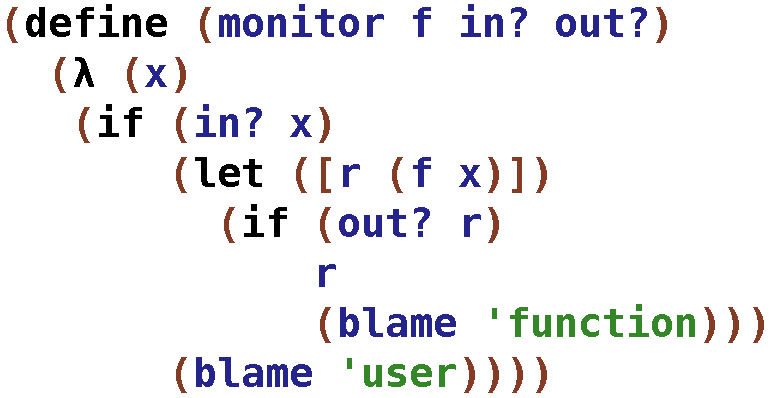
\includegraphics[scale=0.45]{monitor}
 \end{center}

It is well known that wrapping functions like this thwarts the
precision of regular \zcfa{} and higher \kcfa{} as more wrappings are
introduced.
%
In the case of this innocent program
% \begin{alltt}
%   pair(map (monitor to-string int? str?) xs,
%        map (monitor factorial int? int?) xs)
% \end{alltt}
 \begin{center}
  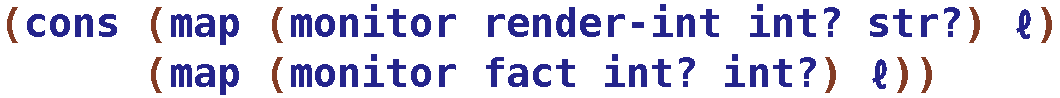
\includegraphics[scale=0.45]{pair}
 \end{center}

according to \zcfa{} the call to the wrapped \texttt{factorial}
function within the second \texttt{map} may return to within the
first \texttt{map}.  Hence \zcfa{} is not sufficiently precise to 
prove \texttt{factorial} cannot be blamed.
%
Using more a context-sensitive analysis such as 1CFA, 2CFA, etc.,
would solve the problem for this example, but would fail for nest
proxies.
%
In general, for any $k$, \kcfa{} will confuse the return flow of some
programs as in this example.
%
Yet, a pushdown abstraction that properly matches calls and returns
has no trouble with this example, regardless of proxy-nesting depth.


%
%% The control cycle from the second \texttt{map} to the first fools state-of-the-art termination checking for untyped higher-order languages~\citep{ianjohnson:DBLP:conf/aplas/SereniJ05}, as it depends on the product of \zcfa{}!
%% %
%% Termination-checking is necessary for interpreting portions of code as their logical equivalents.
%% %
%% Logical interpretations of code let us utilize high-performance theorem provers to test feasability of some code paths for greater precision~\citep{liquid-haskell}.
%% %
%% Functions can become deeply wrapped when interacting through several contracted modules, so pushdown models are nearly a requirement for hope at proving termination.


\paragraph{A systematic approach to pushdown analysis}

At this point, several pushdown analyses for higher-order languages
have been developed~\cite{dvanhorn:Vardoulakis2011CFA2,
dvanhorn:Earl2010Pushdown}, and the basic idea is simple: instead of
approximating a program with a finite state machine, use a pushdown
automata.  The control stack of the automata models the control stack
of the concrete interpreter, while stack frames, which contain
closures, are subject to the same abstraction as values in the
program.

This approach works well for simple languages which obey the stack
discipline of a PDA.  But most languages provide features that
transgress that discipline, such as garbage collection, first-class
control operators, stack inspection, and so on.  Some of these
features have been successfully combined with pushdown analysis, but
required technical innovation and
effort~\cite{dvanhorn:Vardoulakis2011Pushdown,
ianjohnson:DBLP:journals/jfp/JohnsonSEMH14,
dvanhorn:Earl2012Introspective}.  To avoid further one-off efforts, we
develop a general technique for creating pushdown analyses for
languages with control operators and reflective mechanisms.
